\title{Comparison of NBC, LR and SVM for Yelp Review Classification}
\author{Shayan Ali Akbar\\ \small sakbar@purdue.edu\\ \small CS 57300 Homework 3\\
	This is almost a couple of hours late submission.}
\date{}

\documentclass[12pt]{article}
\usepackage{amsmath}
\usepackage[boxruled,linesnumbered]{algorithm2e}
\usepackage{xcolor}
\usepackage{graphicx}

\newcommand\mycommfont[1]{\footnotesize\ttfamily\textcolor{black}{#1}}
\SetCommentSty{mycommfont}

\addtolength{\oddsidemargin}{-.875in}
\addtolength{\evensidemargin}{-.875in}
\addtolength{\textwidth}{1.75in}
\addtolength{\topmargin}{-1.0in}
\addtolength{\textheight}{2.2in}
\pagenumbering{gobble}

\begin{document}
\maketitle

\newpage

\section{Introduction}

In this report we discuss the three very popular classifiers for the task of yelp review
classification. In particular we discuss the naive bayes, logistic regression and support
vector machine classification algorithms.

What follows are the two sections. The next section deals with the Analysis 1 
of the homework 3 handout. And the final section discusses the Analysis 2 of the 
same handout.

\section{Analysis 1}

\subsection{Learning Curves}
The plot of results is shown in Figure 1. On x-axis we vary the training set sizes. Instead
of percents, we have plotted the actual number of training set examples used to learn
the model. On y-axis is the zero one loss. We have three plots --- one for each model.
The blue plot is for logistic regression, the orange for support vector machine, and the
green for naive bayes classifier. The vertical bars show the standard error calculated as
described in the homework handout. The values of zero one loss for each of the six 
training set size averaged accross 10 fold for each of the three models is given below:
\\

average loss for LR = [0.3025, 0.172, 0.123, 0.1045, 0.098, 0.0645]

average loss for SVM = [0.3015, 0.1854, 0.128, 0.1094, 0.1020, 0.073]

average loss for NBC = [0.43499, 0.352, 0.269, 0.2315, 0.1695, 0.1075]
\\

And the respective standard error values are:

standard error for LR = [0.007, 0.0051, 0.0042, 0.0021, 0.00219, 0.001]

standard error for SVM = [0.0075, 0.0049, 0.0039, 0.0026, 0.0023, 0.00143]

standard error for NBC = [0.00570, 0.01027, 0.01323, 0.0112, 0.00736, 0.00448]\\

These average and standard error values are calculated from the following zero
one loss values calculated for each model for training set size for each of the 10 folds.
Notice that the horizontal = bar separated the results for each training set size. The
zero one losses present within two horizontal = bars belong to the different fold for
a specific training set size.\\

\noindent=======================================\\
ZERO-ONE-LOSS-LR 0.26
ZERO-ONE-LOSS-SVM 0.27
ZERO-ONE-LOSS-NBC 0.42
ZERO-ONE-LOSS-LR 0.345
ZERO-ONE-LOSS-SVM 0.335
ZERO-ONE-LOSS-NBC 0.415
ZERO-ONE-LOSS-LR 0.245
ZERO-ONE-LOSS-SVM 0.205
ZERO-ONE-LOSS-NBC 0.465
ZERO-ONE-LOSS-LR 0.295
ZERO-ONE-LOSS-SVM 0.26
ZERO-ONE-LOSS-NBC 0.325
ZERO-ONE-LOSS-LR 0.39
ZERO-ONE-LOSS-SVM 0.41
ZERO-ONE-LOSS-NBC 0.445
ZERO-ONE-LOSS-LR 0.37
ZERO-ONE-LOSS-SVM 0.36
ZERO-ONE-LOSS-NBC 0.36
ZERO-ONE-LOSS-LR 0.245
ZERO-ONE-LOSS-SVM 0.26
ZERO-ONE-LOSS-NBC 0.435
ZERO-ONE-LOSS-LR 0.195
ZERO-ONE-LOSS-SVM 0.2
ZERO-ONE-LOSS-NBC 0.455
ZERO-ONE-LOSS-LR 0.445
ZERO-ONE-LOSS-SVM 0.42
ZERO-ONE-LOSS-NBC 0.52
ZERO-ONE-LOSS-LR 0.235
ZERO-ONE-LOSS-SVM 0.295
ZERO-ONE-LOSS-NBC 0.51\\
=======================================\\
ZERO-ONE-LOSS-LR 0.2
ZERO-ONE-LOSS-SVM 0.27
ZERO-ONE-LOSS-NBC 0.39
ZERO-ONE-LOSS-LR 0.18
ZERO-ONE-LOSS-SVM 0.2
ZERO-ONE-LOSS-NBC 0.44
ZERO-ONE-LOSS-LR 0.175
ZERO-ONE-LOSS-SVM 0.17
ZERO-ONE-LOSS-NBC 0.445
ZERO-ONE-LOSS-LR 0.24
ZERO-ONE-LOSS-SVM 0.22
ZERO-ONE-LOSS-NBC 0.4
ZERO-ONE-LOSS-LR 0.105
ZERO-ONE-LOSS-SVM 0.115
ZERO-ONE-LOSS-NBC 0.12
ZERO-ONE-LOSS-LR 0.12
ZERO-ONE-LOSS-SVM 0.145
ZERO-ONE-LOSS-NBC 0.385
ZERO-ONE-LOSS-LR 0.255
ZERO-ONE-LOSS-SVM 0.245
ZERO-ONE-LOSS-NBC 0.335
ZERO-ONE-LOSS-LR 0.17
ZERO-ONE-LOSS-SVM 0.195
ZERO-ONE-LOSS-NBC 0.36
ZERO-ONE-LOSS-LR 0.185
ZERO-ONE-LOSS-SVM 0.18
ZERO-ONE-LOSS-NBC 0.445
ZERO-ONE-LOSS-LR 0.09
ZERO-ONE-LOSS-SVM 0.115
ZERO-ONE-LOSS-NBC 0.205\\
=======================================\\
ZERO-ONE-LOSS-LR 0.145
ZERO-ONE-LOSS-SVM 0.125
ZERO-ONE-LOSS-NBC 0.35
ZERO-ONE-LOSS-LR 0.115
ZERO-ONE-LOSS-SVM 0.115
ZERO-ONE-LOSS-NBC 0.39
ZERO-ONE-LOSS-LR 0.155
ZERO-ONE-LOSS-SVM 0.165
ZERO-ONE-LOSS-NBC 0.455
ZERO-ONE-LOSS-LR 0.07
ZERO-ONE-LOSS-SVM 0.095
ZERO-ONE-LOSS-NBC 0.23
ZERO-ONE-LOSS-LR 0.115
ZERO-ONE-LOSS-SVM 0.12
ZERO-ONE-LOSS-NBC 0.18
ZERO-ONE-LOSS-LR 0.055
ZERO-ONE-LOSS-SVM 0.065
ZERO-ONE-LOSS-NBC 0.08
ZERO-ONE-LOSS-LR 0.115
ZERO-ONE-LOSS-SVM 0.115
ZERO-ONE-LOSS-NBC 0.185
ZERO-ONE-LOSS-LR 0.115
ZERO-ONE-LOSS-SVM 0.135
ZERO-ONE-LOSS-NBC 0.19
ZERO-ONE-LOSS-LR 0.215
ZERO-ONE-LOSS-SVM 0.22
ZERO-ONE-LOSS-NBC 0.485
ZERO-ONE-LOSS-LR 0.135
ZERO-ONE-LOSS-SVM 0.125
ZERO-ONE-LOSS-NBC 0.15\\
=======================================\\
ZERO-ONE-LOSS-LR 0.08
ZERO-ONE-LOSS-SVM 0.075
ZERO-ONE-LOSS-NBC 0.06
ZERO-ONE-LOSS-LR 0.095
ZERO-ONE-LOSS-SVM 0.1
ZERO-ONE-LOSS-NBC 0.135
ZERO-ONE-LOSS-LR 0.115
ZERO-ONE-LOSS-SVM 0.125
ZERO-ONE-LOSS-NBC 0.415
ZERO-ONE-LOSS-LR 0.085
ZERO-ONE-LOSS-SVM 0.085
ZERO-ONE-LOSS-NBC 0.075
ZERO-ONE-LOSS-LR 0.105
ZERO-ONE-LOSS-SVM 0.105
ZERO-ONE-LOSS-NBC 0.2
ZERO-ONE-LOSS-LR 0.1
ZERO-ONE-LOSS-SVM 0.1
ZERO-ONE-LOSS-NBC 0.275
ZERO-ONE-LOSS-LR 0.075
ZERO-ONE-LOSS-SVM 0.095
ZERO-ONE-LOSS-NBC 0.23
ZERO-ONE-LOSS-LR 0.145
ZERO-ONE-LOSS-SVM 0.175
ZERO-ONE-LOSS-NBC 0.28
ZERO-ONE-LOSS-LR 0.115
ZERO-ONE-LOSS-SVM 0.115
ZERO-ONE-LOSS-NBC 0.385
ZERO-ONE-LOSS-LR 0.13
ZERO-ONE-LOSS-SVM 0.12
ZERO-ONE-LOSS-NBC 0.26\\
=======================================\\
ZERO-ONE-LOSS-LR 0.1
ZERO-ONE-LOSS-SVM 0.11
ZERO-ONE-LOSS-NBC 0.26
ZERO-ONE-LOSS-LR 0.065
ZERO-ONE-LOSS-SVM 0.08
ZERO-ONE-LOSS-NBC 0.07
ZERO-ONE-LOSS-LR 0.095
ZERO-ONE-LOSS-SVM 0.09
ZERO-ONE-LOSS-NBC 0.125
ZERO-ONE-LOSS-LR 0.07
ZERO-ONE-LOSS-SVM 0.075
ZERO-ONE-LOSS-NBC 0.12
ZERO-ONE-LOSS-LR 0.145
ZERO-ONE-LOSS-SVM 0.145
ZERO-ONE-LOSS-NBC 0.225
ZERO-ONE-LOSS-LR 0.1
ZERO-ONE-LOSS-SVM 0.115
ZERO-ONE-LOSS-NBC 0.24
ZERO-ONE-LOSS-LR 0.115
ZERO-ONE-LOSS-SVM 0.095
ZERO-ONE-LOSS-NBC 0.095
ZERO-ONE-LOSS-LR 0.115
ZERO-ONE-LOSS-SVM 0.115
ZERO-ONE-LOSS-NBC 0.23
ZERO-ONE-LOSS-LR 0.085
ZERO-ONE-LOSS-SVM 0.075
ZERO-ONE-LOSS-NBC 0.25
ZERO-ONE-LOSS-LR 0.1
ZERO-ONE-LOSS-SVM 0.12
ZERO-ONE-LOSS-NBC 0.08\\
=======================================\\
ZERO-ONE-LOSS-LR 0.055
ZERO-ONE-LOSS-SVM 0.06
ZERO-ONE-LOSS-NBC 0.19
ZERO-ONE-LOSS-LR 0.09
ZERO-ONE-LOSS-SVM 0.1
ZERO-ONE-LOSS-NBC 0.065
ZERO-ONE-LOSS-LR 0.04
ZERO-ONE-LOSS-SVM 0.08
ZERO-ONE-LOSS-NBC 0.15
ZERO-ONE-LOSS-LR 0.07
ZERO-ONE-LOSS-SVM 0.08
ZERO-ONE-LOSS-NBC 0.115
ZERO-ONE-LOSS-LR 0.095
ZERO-ONE-LOSS-SVM 0.085
ZERO-ONE-LOSS-NBC 0.155
ZERO-ONE-LOSS-LR 0.065
ZERO-ONE-LOSS-SVM 0.08
ZERO-ONE-LOSS-NBC 0.065
ZERO-ONE-LOSS-LR 0.07
ZERO-ONE-LOSS-SVM 0.06
ZERO-ONE-LOSS-NBC 0.085
ZERO-ONE-LOSS-LR 0.045
ZERO-ONE-LOSS-SVM 0.06
ZERO-ONE-LOSS-NBC 0.055
ZERO-ONE-LOSS-LR 0.05
ZERO-ONE-LOSS-SVM 0.05
ZERO-ONE-LOSS-NBC 0.13
ZERO-ONE-LOSS-LR 0.065
ZERO-ONE-LOSS-SVM 0.075
ZERO-ONE-LOSS-NBC 0.065\\


\begin{figure}
	\centering
	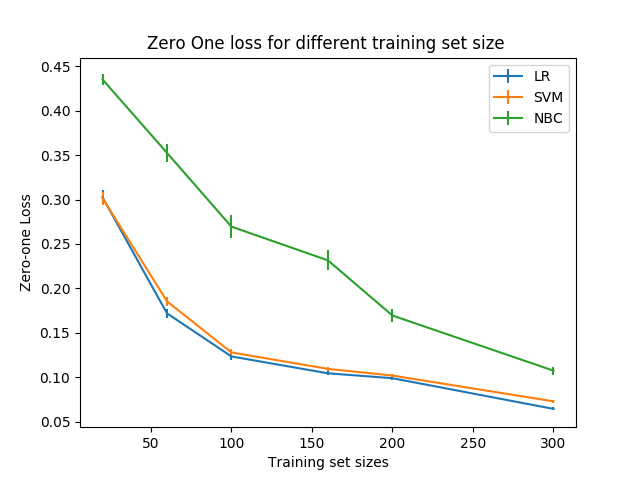
\includegraphics{AllModelsBinaryFeats.png}
\end{figure}

\subsection{Hypothesis}

Let's compare the two algorithms LR and NBC. 

Null hypothesis is that the LR and NBC are equivalent in terms of performance. It is assumed
to be true. While the alternative hypothesis is that LR and NBC zero one losses are significantly different.

\subsection{Discussion to test the hypothesis}

It is obvious from the plot of Figure 1 of average zero one losses and standard errors of the two
algorithms (LR and NBC) that their performances are very different from each other. This is because
in none of the training set sizes the error bars in the plot for the two algorithms are overlapping
each other as the plots are very far apart from each other.

Nonetheless we perform paired t-test to compare their performances and to figure out whether
the differences between performances are statistically significant. The t-test are performed using
online tool called GraphPad. Following are the results for each training set size.\\

For 1\% training set size:
  The two-tailed P value equals 0.0025 which is less than $\alpha$ = 0.05.
  This difference is considered to be statistically significant. 
  The mean of LR minus NBC equals -0.13250.
  95\% confidence interval of this difference: From -0.20495 to -0.06005 \\

For 3\% training set size:
  The two-tailed P value equals 0.0001  which is less than $\alpha$ = 0.05.
  This difference is considered to be statistically significant. 
  The mean of LR minus NBC equals -0.18050 .
  95\% confidence interval of this difference: From -0.24367 to -0.11733 \\

For 5\% training set size:
  The two-tailed P value equals 0.0023  which is less than $\alpha$ = 0.05.
  This difference is considered to be statistically significant. 
  The mean of LR minus NBC equals -0.14600.
  95\% confidence interval of this difference: From -0.22458 to -0.06742  \\

For 8\% training set size:
  The two-tailed P value equals 0.0045  which is less than $\alpha$ = 0.05.
  This difference is considered to be statistically significant. 
  The mean of LR minus NBC equals -0.12700 
  95\% confidence interval of this difference: From -0.20335 to -0.05065 \\

For 10\% training set size:
  The two-tailed P value equals 0.0127  which is less than $\alpha$ = 0.05.
  This difference is considered to be statistically significant. 
  The mean of LR minus NBC equals -0.07050 
  95\% confidence interval of this difference: From -0.12196 to -0.01904 \\

For 15\% training set size:
  The two-tailed P value equals 0.0292  which is less than $\alpha$ = 0.05.
  This difference is considered to be statistically significant. 
  The mean of LR minus NBC equals  -0.04300 
  95\% confidence interval of this difference: From -0.08056 to -0.00544  \\

Since the difference of the zero one losses for the two algorithms are statistically significant
for all the training set sizes, we conclude that the alternative hypothesis is true and null 
hypothesis is rejected.

\section{Analysis 2}

\subsection{Learning Curves}

Adding one more value to the feature to make it three value, we perform the experiments
for the three models (LR, SVM, and NBC) and plot the reuslting learning curves as shown in
Figure 2.

 On x-axis we vary the training set sizes. Instead of percents, we have plotted the actual
 number of training set examples used to learn the model. On y-axis is the zero one loss. 
We have three plots --- one for each model. The blue plot is for logistic regression, the 
orange for support vector machine, and the green for naive bayes classifier. The vertical 
bars show the standard error calculated as described in the homework handout. The 
values of zero one loss for each of the six training set size averaged accross 10 fold for 
each of the three models is given below:
\\

=======LR======

avg = [0.3125, 0.169, 0.1259, 0.0905, 
0.08149, 0.06299]

se = [0.00822, 0.0021, 
0.00174, 0.0018, 
0.002214, 0.00148]

=======SVM======

avg=[0.3170, 0.1635, 0.1389, 0.101, 
0.087, 0.0725]

se = [0.006438, 0.0024601, 
0.002457, 0.00304, 
0.001584, 0.00184]

=======NBC======

avg = [0.4779999, 0.4255, 0.3889, 0.3355, 
0.276499, 0.177]

se  = [0.0067, 0.008664, 
0.0069, 0.010, 
0.0093, 0.008]

=======LR2val======

avg = [0.3290, 0.1859, 0.136, 0.0915, 
0.083, 0.075]

se = [0.007986, 0.00254, 
0.00178, 0.0018, 
0.00152, 0.0011]
\\

The above values are calculated from the following zero one loss values for varying training
set size each having10 folds:
\\

=======================================\\
ZERO-ONE-LOSS-LR 0.2
ZERO-ONE-LOSS-LR-2val 0.27
ZERO-ONE-LOSS-SVM 0.275
ZERO-ONE-LOSS-NBC 0.57
ZERO-ONE-LOSS-LR 0.41
ZERO-ONE-LOSS-LR-2val 0.41
ZERO-ONE-LOSS-SVM 0.355
ZERO-ONE-LOSS-NBC 0.495
ZERO-ONE-LOSS-LR 0.445
ZERO-ONE-LOSS-LR-2val 0.47
ZERO-ONE-LOSS-SVM 0.405
ZERO-ONE-LOSS-NBC 0.48
ZERO-ONE-LOSS-LR 0.32
ZERO-ONE-LOSS-LR-2val 0.34
ZERO-ONE-LOSS-SVM 0.31
ZERO-ONE-LOSS-NBC 0.455
ZERO-ONE-LOSS-LR 0.21
ZERO-ONE-LOSS-LR-2val 0.255
ZERO-ONE-LOSS-SVM 0.205
ZERO-ONE-LOSS-NBC 0.47
ZERO-ONE-LOSS-LR 0.295
ZERO-ONE-LOSS-LR-2val 0.265
ZERO-ONE-LOSS-SVM 0.35
ZERO-ONE-LOSS-NBC 0.38
ZERO-ONE-LOSS-LR 0.285
ZERO-ONE-LOSS-LR-2val 0.27
ZERO-ONE-LOSS-SVM 0.27
ZERO-ONE-LOSS-NBC 0.55
ZERO-ONE-LOSS-LR 0.41
ZERO-ONE-LOSS-LR-2val 0.45
ZERO-ONE-LOSS-SVM 0.41
ZERO-ONE-LOSS-NBC 0.5
ZERO-ONE-LOSS-LR 0.23
ZERO-ONE-LOSS-LR-2val 0.255
ZERO-ONE-LOSS-SVM 0.245
ZERO-ONE-LOSS-NBC 0.345
ZERO-ONE-LOSS-LR 0.32
ZERO-ONE-LOSS-LR-2val 0.305
ZERO-ONE-LOSS-SVM 0.345
ZERO-ONE-LOSS-NBC 0.535\\

=======================================\\

ZERO-ONE-LOSS-LR 0.16
ZERO-ONE-LOSS-LR-2val 0.165
ZERO-ONE-LOSS-SVM 0.185
ZERO-ONE-LOSS-NBC 0.56
ZERO-ONE-LOSS-LR 0.135
ZERO-ONE-LOSS-LR-2val 0.155
ZERO-ONE-LOSS-SVM 0.135
ZERO-ONE-LOSS-NBC 0.42
ZERO-ONE-LOSS-LR 0.205
ZERO-ONE-LOSS-LR-2val 0.205
ZERO-ONE-LOSS-SVM 0.2
ZERO-ONE-LOSS-NBC 0.475
ZERO-ONE-LOSS-LR 0.195
ZERO-ONE-LOSS-LR-2val 0.22
ZERO-ONE-LOSS-SVM 0.175
ZERO-ONE-LOSS-NBC 0.49
ZERO-ONE-LOSS-LR 0.17
ZERO-ONE-LOSS-LR-2val 0.195
ZERO-ONE-LOSS-SVM 0.155
ZERO-ONE-LOSS-NBC 0.37
ZERO-ONE-LOSS-LR 0.18
ZERO-ONE-LOSS-LR-2val 0.235
ZERO-ONE-LOSS-SVM 0.175
ZERO-ONE-LOSS-NBC 0.45
ZERO-ONE-LOSS-LR 0.14
ZERO-ONE-LOSS-LR-2val 0.16
ZERO-ONE-LOSS-SVM 0.12
ZERO-ONE-LOSS-NBC 0.34
ZERO-ONE-LOSS-LR 0.165
ZERO-ONE-LOSS-LR-2val 0.175
ZERO-ONE-LOSS-SVM 0.18
ZERO-ONE-LOSS-NBC 0.495
ZERO-ONE-LOSS-LR 0.185
ZERO-ONE-LOSS-LR-2val 0.17
ZERO-ONE-LOSS-SVM 0.175
ZERO-ONE-LOSS-NBC 0.415
ZERO-ONE-LOSS-LR 0.155
ZERO-ONE-LOSS-LR-2val 0.18
ZERO-ONE-LOSS-SVM 0.135
ZERO-ONE-LOSS-NBC 0.24\\

=======================================\\

ZERO-ONE-LOSS-LR 0.11
ZERO-ONE-LOSS-LR-2val 0.15
ZERO-ONE-LOSS-SVM 0.115
ZERO-ONE-LOSS-NBC 0.405
ZERO-ONE-LOSS-LR 0.125
ZERO-ONE-LOSS-LR-2val 0.11
ZERO-ONE-LOSS-SVM 0.13
ZERO-ONE-LOSS-NBC 0.385
ZERO-ONE-LOSS-LR 0.11
ZERO-ONE-LOSS-LR-2val 0.11
ZERO-ONE-LOSS-SVM 0.13
ZERO-ONE-LOSS-NBC 0.445
ZERO-ONE-LOSS-LR 0.16
ZERO-ONE-LOSS-LR-2val 0.16
ZERO-ONE-LOSS-SVM 0.205
ZERO-ONE-LOSS-NBC 0.44
ZERO-ONE-LOSS-LR 0.135
ZERO-ONE-LOSS-LR-2val 0.13
ZERO-ONE-LOSS-SVM 0.135
ZERO-ONE-LOSS-NBC 0.425
ZERO-ONE-LOSS-LR 0.125
ZERO-ONE-LOSS-LR-2val 0.145
ZERO-ONE-LOSS-SVM 0.115
ZERO-ONE-LOSS-NBC 0.37
ZERO-ONE-LOSS-LR 0.105
ZERO-ONE-LOSS-LR-2val 0.12
ZERO-ONE-LOSS-SVM 0.135
ZERO-ONE-LOSS-NBC 0.205
ZERO-ONE-LOSS-LR 0.11
ZERO-ONE-LOSS-LR-2val 0.13
ZERO-ONE-LOSS-SVM 0.13
ZERO-ONE-LOSS-NBC 0.445
ZERO-ONE-LOSS-LR 0.13
ZERO-ONE-LOSS-LR-2val 0.16
ZERO-ONE-LOSS-SVM 0.14
ZERO-ONE-LOSS-NBC 0.345
ZERO-ONE-LOSS-LR 0.15
ZERO-ONE-LOSS-LR-2val 0.145
ZERO-ONE-LOSS-SVM 0.155
ZERO-ONE-LOSS-NBC 0.425\\

=======================================\\

ZERO-ONE-LOSS-LR 0.085
ZERO-ONE-LOSS-LR-2val 0.085
ZERO-ONE-LOSS-SVM 0.1
ZERO-ONE-LOSS-NBC 0.255
ZERO-ONE-LOSS-LR 0.105
ZERO-ONE-LOSS-LR-2val 0.095
ZERO-ONE-LOSS-SVM 0.11
ZERO-ONE-LOSS-NBC 0.37
ZERO-ONE-LOSS-LR 0.05
ZERO-ONE-LOSS-LR-2val 0.05
ZERO-ONE-LOSS-SVM 0.04
ZERO-ONE-LOSS-NBC 0.26
ZERO-ONE-LOSS-LR 0.065
ZERO-ONE-LOSS-LR-2val 0.075
ZERO-ONE-LOSS-SVM 0.07
ZERO-ONE-LOSS-NBC 0.065
ZERO-ONE-LOSS-LR 0.085
ZERO-ONE-LOSS-LR-2val 0.09
ZERO-ONE-LOSS-SVM 0.16
ZERO-ONE-LOSS-NBC 0.38
ZERO-ONE-LOSS-LR 0.105
ZERO-ONE-LOSS-LR-2val 0.11
ZERO-ONE-LOSS-SVM 0.105
ZERO-ONE-LOSS-NBC 0.395
ZERO-ONE-LOSS-LR 0.105
ZERO-ONE-LOSS-LR-2val 0.095
ZERO-ONE-LOSS-SVM 0.115
ZERO-ONE-LOSS-NBC 0.37
ZERO-ONE-LOSS-LR 0.095
ZERO-ONE-LOSS-LR-2val 0.09
ZERO-ONE-LOSS-SVM 0.125
ZERO-ONE-LOSS-NBC 0.37
ZERO-ONE-LOSS-LR 0.1
ZERO-ONE-LOSS-LR-2val 0.11
ZERO-ONE-LOSS-SVM 0.085
ZERO-ONE-LOSS-NBC 0.43
ZERO-ONE-LOSS-LR 0.11
ZERO-ONE-LOSS-LR-2val 0.115
ZERO-ONE-LOSS-SVM 0.1
ZERO-ONE-LOSS-NBC 0.46\\

=======================================\\

ZERO-ONE-LOSS-LR 0.115
ZERO-ONE-LOSS-LR-2val 0.11
ZERO-ONE-LOSS-SVM 0.1
ZERO-ONE-LOSS-NBC 0.31
ZERO-ONE-LOSS-LR 0.075
ZERO-ONE-LOSS-LR-2val 0.075
ZERO-ONE-LOSS-SVM 0.09
ZERO-ONE-LOSS-NBC 0.33
ZERO-ONE-LOSS-LR 0.04
ZERO-ONE-LOSS-LR-2val 0.06
ZERO-ONE-LOSS-SVM 0.055
ZERO-ONE-LOSS-NBC 0.275
ZERO-ONE-LOSS-LR 0.09
ZERO-ONE-LOSS-LR-2val 0.085
ZERO-ONE-LOSS-SVM 0.11
ZERO-ONE-LOSS-NBC 0.255
ZERO-ONE-LOSS-LR 0.105
ZERO-ONE-LOSS-LR-2val 0.095
ZERO-ONE-LOSS-SVM 0.095
ZERO-ONE-LOSS-NBC 0.355
ZERO-ONE-LOSS-LR 0.08
ZERO-ONE-LOSS-LR-2val 0.09
ZERO-ONE-LOSS-SVM 0.09
ZERO-ONE-LOSS-NBC 0.105
ZERO-ONE-LOSS-LR 0.1
ZERO-ONE-LOSS-LR-2val 0.09
ZERO-ONE-LOSS-SVM 0.1
ZERO-ONE-LOSS-NBC 0.375
ZERO-ONE-LOSS-LR 0.085
ZERO-ONE-LOSS-LR-2val 0.1
ZERO-ONE-LOSS-SVM 0.085
ZERO-ONE-LOSS-NBC 0.375
ZERO-ONE-LOSS-LR 0.075
ZERO-ONE-LOSS-LR-2val 0.07
ZERO-ONE-LOSS-SVM 0.08
ZERO-ONE-LOSS-NBC 0.11
ZERO-ONE-LOSS-LR 0.05
ZERO-ONE-LOSS-LR-2val 0.065
ZERO-ONE-LOSS-SVM 0.065
ZERO-ONE-LOSS-NBC 0.275\\

=======================================\\

ZERO-ONE-LOSS-LR 0.05
ZERO-ONE-LOSS-LR-2val 0.06
ZERO-ONE-LOSS-SVM 0.065
ZERO-ONE-LOSS-NBC 0.15
ZERO-ONE-LOSS-LR 0.065
ZERO-ONE-LOSS-LR-2val 0.085
ZERO-ONE-LOSS-SVM 0.065
ZERO-ONE-LOSS-NBC 0.23
ZERO-ONE-LOSS-LR 0.045
ZERO-ONE-LOSS-LR-2val 0.06
ZERO-ONE-LOSS-SVM 0.045
ZERO-ONE-LOSS-NBC 0.135
ZERO-ONE-LOSS-LR 0.06
ZERO-ONE-LOSS-LR-2val 0.09
ZERO-ONE-LOSS-SVM 0.075
ZERO-ONE-LOSS-NBC 0.12
ZERO-ONE-LOSS-LR 0.095
ZERO-ONE-LOSS-LR-2val 0.075
ZERO-ONE-LOSS-SVM 0.085
ZERO-ONE-LOSS-NBC 0.16
ZERO-ONE-LOSS-LR 0.075
ZERO-ONE-LOSS-LR-2val 0.075
ZERO-ONE-LOSS-SVM 0.08
ZERO-ONE-LOSS-NBC 0.1
ZERO-ONE-LOSS-LR 0.045
ZERO-ONE-LOSS-LR-2val 0.07
ZERO-ONE-LOSS-SVM 0.055
ZERO-ONE-LOSS-NBC 0.145
ZERO-ONE-LOSS-LR 0.055
ZERO-ONE-LOSS-LR-2val 0.06
ZERO-ONE-LOSS-SVM 0.06
ZERO-ONE-LOSS-NBC 0.23
ZERO-ONE-LOSS-LR 0.075
ZERO-ONE-LOSS-LR-2val 0.09
ZERO-ONE-LOSS-SVM 0.115
ZERO-ONE-LOSS-NBC 0.09
ZERO-ONE-LOSS-LR 0.065
ZERO-ONE-LOSS-LR-2val 0.085
ZERO-ONE-LOSS-SVM 0.08
ZERO-ONE-LOSS-NBC 0.41\\



\begin{figure}
	\centering
	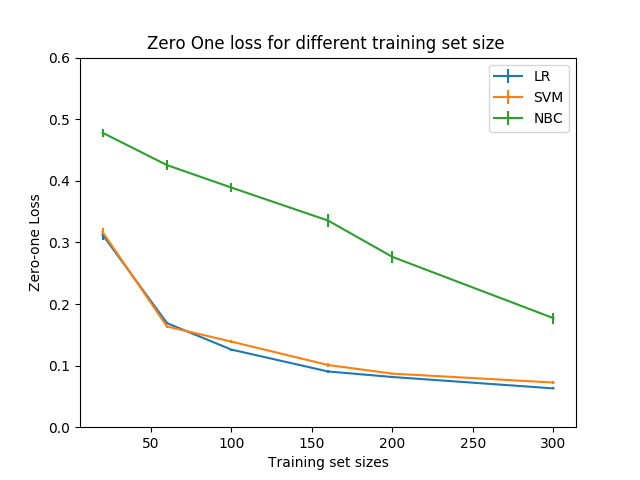
\includegraphics{AllModelsThreeFeats.png}
\end{figure}

\subsection{Hypothesis}

Let's compare Logistic regression which uses three features (LR-3val) with
 Logistic regression which uses two features (LR-2val).

Null hypothesis is that both are equivalent in terms of performance. It is assumed
to be true. While the alternative hypothesis is that LR-3val and LR-2val zero one losses 
are significantly different.


\subsection{Discussion to test the hypothesis}

It can be seen from the average zero one loss and standard error values for LR-3val and LR-2val
that the difference is not significant. The standard error values for LR-3val do not overlap with the
LR-Binary values.

We perform t-test to compare the performance. The results for different training set sizes are given below:

For 1\% training set size:
  The two-tailed P value equals 0.1296  which is greater than $\alpha$ = 0.05.
  This difference is considered to be NOT statistically significant. 
  The mean of LR-3val minus LR-2val equals  -0.01650 .
  95\% confidence interval of this difference: From -0.03887 to 0.00587  \\

For 3\% training set size:
  The two-tailed P value equals 0.0185  which is less than $\alpha$ = 0.05.
  This difference is considered to be statistically significant. 
  The mean of LR-3val minus LR-2val  equals -0.01700 .
  95\% confidence interval of this difference: From -0.03040 to -0.00360  \\

For 5\% training set size:
  The two-tailed P value equals 0.1066  which is greater than $\alpha$ = 0.05.
  This difference is considered to be NOT statistically significant. 
  The mean of  LR-3val minus LR-2val  equals   -0.01000 .
  95\% confidence interval of this difference: From -0.02262 to 0.00262   \\

For 8\% training set size:
  The two-tailed P value equals 0.6783   which is greater than $\alpha$ = 0.05.
  This difference is considered to be NOT statistically significant. 
  The mean of LR-3val minus LR-2val  equals  -0.00100 
  95\% confidence interval of this difference: From -0.00628 to 0.00428 \\

For 10\% training set size:
  The two-tailed P value equals 0.5042  which is greater than $\alpha$ = 0.05.
  This difference is considered to be NOT statistically significant. 
  The mean of  LR-3val minus LR-2val  equals  -0.00250 . 
  95\% confidence interval of this difference: From -0.01063 to 0.00563  \\

For 15\% training set size:
  The two-tailed P value equals 0.0269  which is less than $\alpha$ = 0.05.
  This difference is considered to be statistically significant. 
  The mean of  LR-3val minus LR-2val  equals -0.01200
  95\% confidence interval of this difference: From -0.02228 to -0.00172   \\

Since the differences of zero one losses for all the training set sizes (except for 3 and 15\%)
are NOT statistically significant we conclude that the addition of a new feature
does not enhance the algorithm much and the results are comparable. Null hypothesis
is true in this case and we accept it.

\end{document}